%%%%%%%%%%%%%%%%%%%%%%%%%%%%%%%%%%%%%%%%%%%%%%%%%%%%%%%%%%%%%%%%%%%%%%%%%%%%
%% Trim Size: 9.75in x 6.5in
%% Text Area: 8in (include Runningheads) x 5in
%% ws-ijmpc.tex:   18-02-2020
%% Tex file to use with ws-ijmpc.cls written in Latex2E.
%% The content, structure, format and layout of this style file is the
%% property of World Scientific Publishing Co. Pte. Ltd.
%% Copyright 2014 by World Scientific Publishing Co.
%% All rights are reserved.
%%%%%%%%%%%%%%%%%%%%%%%%%%%%%%%%%%%%%%%%%%%%%%%%%%%%%%%%%%%%%%%%%%%%%%%%%%%%
%
%\documentclass[draft]{ws-ijmpc}
\documentclass{ws-ijmpc}
\usepackage[super]{cite} % other options `nocompress`, `nosort`
\begin{document}

\markboth{F. Author \& S. Author (authors' names)}
{Instructions for typing manuscripts (paper's title)}

%%%%%%%%%%%%%%%%%%%%% Publisher's Area please ignore %%%%%%%%%%%%%%%
\catchline{}{}{}{}{}
%%%%%%%%%%%%%%%%%%%%%%%%%%%%%%%%%%%%%%%%%%%%%%%%%%%%%%%%%%%%%%%%%%%%

\title{Instructions for typesetting
manuscripts\footnote{For the title, try not to use more than
3 lines. Typeset the title in 10~pt Roman, sentence case and
boldface.}
}

\author{First Author\footnote{
Typeset names in 8~pt Roman, upper and lower case. Use the footnote to indicate the
present or permanent address of the author.}}

\address{University Department, University Name, Address\\
City, State ZIP/Zone,
Country\footnote{State completely without abbreviations, the
affiliation and mailing address, including country. Typeset in 8~pt
italic.}\\
first\_author@domain\_name}

\author{Second Author}

\address{Group, Laboratory, Address\\
City, State ZIP/Zone, Country\\
second\_author@domain\_name}

\maketitle

\begin{history}
\received{Day Month Year}
\revised{Day Month Year}
\end{history}

\begin{abstract}
The abstract should summarize the context, content
and conclusions of the paper in less than 200 words. It should
not contain any references or displayed equations. Typeset the
abstract in 8 pt Roman with baselineskip of 10 pt, making
an indentation of 1.5 pica on the left and right margins.

\keywords{Four or five keywords; separated by semicolon.}
\end{abstract}

\ccode{PACS Nos.:}

\section{The Main Text}

Contributions to the {\it International Journal of Modern Physics C\/}
are to be in\break
English. Authors are encouraged to have their
contribution checked for grammar. American spelling should be
used. Abbreviations are allowed but should be spelt out in full when
first used. Integers ten and below are to be spelt out. Italicize
foreign language phrases (e.g.,~Latin, French).

The text is to be typeset in 10 pt Roman, single spaced with
baselineskip of 13~pt. Text area (including copyright block)
is 8 inches high and 5 inches wide for the first page.  Text area
(excluding running title) is 7.7 inches high and 5 inches wide for
subsequent pages.  Final pagination and insertion of running titles
will be done by the publisher.

\section{Major Headings}

Major headings should be typeset in boldface with the first
letter of important words capitalized.

\subsection{Sub-headings}

Sub-headings should be typeset in boldface italic and capitalize
the first letter of the first word only. Section number to be in
boldface Roman.

\subsubsection{Sub-subheadings}

Typeset sub-subheadings in medium face italic and capitalize the
first letter of the first word only. Section numbers to be in
roman.

\subsection{Numbering and spacing}

Sections, sub-sections and sub-subsections are numbered in
Arabic.  Use double spacing before all section headings, and
single spacing after section headings. Flush left all paragraphs
that follow after section headings.

\subsection{Lists of items}

Lists may be laid out with each item marked by a dot:
\begin{itemlist}
 \item item one,
 \item item two.
\end{itemlist}
Items may also be numbered in lowercase Roman numerals:
\begin{romanlist}[(ii)]
\item item one
\item item two
	\begin{romanlist}[(b)]
	\item lists within lists can be numbered with lowercase
              Roman letters,
	\item second item.
	\end{romanlist}
\end{romanlist}

\section{Equations}

Displayed equations should be numbered consecutively in the whole
paper, with the number set flush right and enclosed in
parentheses
\begin{equation}
\mu(n, t) = \frac{\sum^\infty_{i=1} 1(d_i < t, N(d_i)
= n)}{\int^t_{\sigma=0} 1(N(\sigma) = n)d\sigma}\,.
\label{diseqn}
\end{equation}

Equations should be referred to in abbreviated form,
e.g.,~``Eq.~(\ref{diseqn})'' or ``(2)''. In multiple-line
equations, the number should be given on the last line.

Displayed equations are to be centered on the page width.
Standard English letters like x are to appear as $x$
(italicized) in the text if they are used as mathematical
symbols. Punctuation marks are used at the end of equations as
if they appeared directly in the text.

\begin{theorem}
Theorems$,$ lemmas$,$ etc. are to be numbered
consecutively in the paper. Use double spacing before and after
theorems, lemmas, etc.
\end{theorem}

\begin{proof}
The word `Proof' should be type in boldface. Proofs
should end with\break
a box.
\end{proof}

\section{Illustrations and Photographs}
Figures are to be inserted in the text nearest their first
reference. If the author requires the publisher to reduce the figures,
ensure that the figures (including letterings and numbers) are large
enough to be clearly seen after reduction. If photographs are to be
used, only black and white ones are acceptable.

\begin{figure}[ph]
\centerline{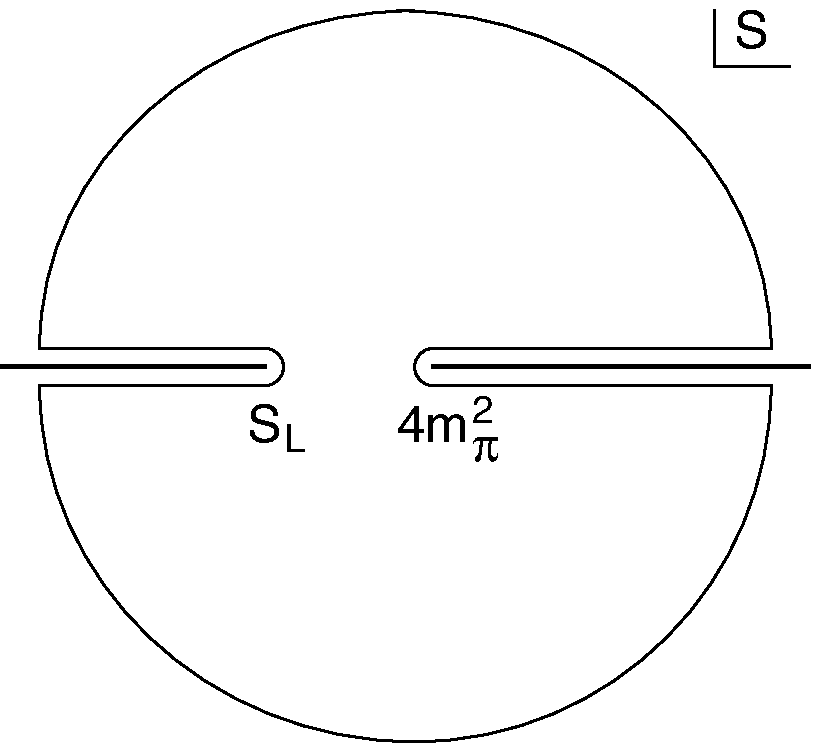
\includegraphics[width=4.7cm]{ijmpcf1}}
\vspace*{8pt}
\caption{A schematic illustration of dissociative recombination. The
direct mechanism, 4m$^2_\pi$ is initiated when the
molecular ion S$_{\rm L}$ captures an electron with
kinetic energy. \label{f1}}
\end{figure}

Figures are to be sequentially numbered in Arabic numerals. The
caption must be placed below the figure (see Fig.~\ref{f1}). Typeset
in 8 pt Roman with baselineskip of 10~pt. Use double spacing
between a caption and the text that follows immediately.

Previously published material must be accompanied by written
permission from the author and publisher.

\section{Tables}

Tables should be inserted in the text as close to the point of
reference as possible. Some space should be left above and below
the table.

Tables should be numbered sequentially in the text in Arabic
numerals. Captions are to be centralized above the tables.
Typeset tables and captions in 8 pt Roman with
baselineskip of 10 pt.

\begin{table}[ht]
\tbl{Comparison of acoustic for frequencies for piston-cylinder problem.}
{\begin{tabular}{@{}cccc@{}} \toprule
Piston mass & Analytical frequency & TRIA6-$S_1$ model &
\% Error \\
& (Rad/s) & (Rad/s) \\ \colrule
1.0\hphantom{00} & \hphantom{0}281.0 & \hphantom{0}280.81 & 0.07 \\
0.1\hphantom{00} & \hphantom{0}876.0 & \hphantom{0}875.74 & 0.03 \\
0.01\hphantom{0} & 2441.0 & 2441.0\hphantom{0} & 0.0\hphantom{0} \\
0.001 & 4130.0 & 4129.3\hphantom{0} & 0.16\\ \botrule
\end{tabular} \label{ta1}}
\end{table}

If tables need to extend over to a second page, the continuation of
the table should be preceded by a caption, e.g.,~``{\it Table 2.}
$(${\it Continued}$)$''.

\section{Footnotes}
Footnotes should be numbered sequentially in superscript
lowercase Roman letters.\footnote{Footnotes should be
typeset in 8 pt Roman at the bottom of the page.}

\section{References}
References are to be listed in the order cited in the text in Arabic
numerals.  They can be typed in superscripts after punctuation marks,
e.g.,~``$\ldots$ in the statement.\cite{1,2,3}'' or used directly,
e.g.,~``see Ref.~\citen{4} for examples''. Please list using the
style shown in the following examples.  For journal names, use the
standard abbreviations or spell in full. Typeset the references in 9 pt
roman with baselineskip of 11 pt.

\section*{Acknowledgments}
This section should come before the References. Dedications and
funding information may also be included here.

\appendix

\section{Appendices}
Appendices should be used only when absolutely necessary. They
should come before the References. If there is more than one
appendix, number them alphabetically. Number displayed equations
occurring in the Appendix in this way, e.g.~(\ref{app1}),\break
(\ref{app2}), etc.
\begin{eqnarray}	%A.1
\begin{array}{rcl}
g_{\mu_1\mu_2} &=& g_{axby}=-\displaystyle{\epsilon_{abc}}{4\pi}\,
\frac{(x-y)^c}{|x-y|^3}\,, \\[8pt]
h_{\mu_1\mu_2\mu_3} &=& \epsilon^{\alpha_1 \alpha_2 \alpha_3}
g_{\mu_1\alpha_1}g_{\mu_2\alpha_2}g_{\mu_3\alpha_3}
\end{array}
\label{app1}
\end{eqnarray}
with
\begin{eqnarray}	%A.2
\epsilon^{\alpha_1 \alpha_2 \alpha_3} = \epsilon^{b_1y_1b_2y_2cx} =
\epsilon^{b_1b_2c}\delta(x-y_1)\delta(x-y_2)\,.
\label{app2}
\end{eqnarray}

%\begin{thebibliography}{000} %for 3 digits
%\begin{thebibliography}{00}  %for 2 digits
%\begin{thebibliography}{0}   %for 1 digit

\begin{thebibliography}{0}
\bibitem{1} J. Callaway, {\it Phys. Rev. B} {\bf 35}, 8723 (1987).

\bibitem{2} M. Tinkham, {\it Group Theory and Quantum Mechanics}
(McGraw-Hill, New York, 1964).

\bibitem{3} T. Tel, {\it Experimental Study and Characterization
of Chaos}, ed. Hao Bailin (World Scientific, Singapore, 1990), p. 149.

\bibitem{4} P. P. Edwards, {\it Superconductivity and
Applications --- Proc. Taiwan Int. Symp. Superconductivity},
ed.~P. T. Wu {\it et al.} (World Scientific, Singapore, 1989), p. 29.

\bibitem{5} W. J. Johnson, Ph.D. thesis, University of Wisconsin,
Madison (1968).

\bibitem{6} P. F. Marteau and H. D. I. Arbabanel, Noise reduction in
chaotic time series using scaled probabilistic methods, UCSD/INLS
preprint, October 1990.

\bibitem{7} J. D. Jackson, {\it Classical Electrodynamics} (Wiley,
New York, 1963), p.~93.

\bibitem{8} J. Jeans, {\it The Mathematical Theory of Electricity
and Magnetism} (Cambridge University Press, 1963), p.~249.
\end{thebibliography}

\end{document} 